\section{Hintergrund und Verwandte Arbeiten}

\subsection{Angry Birds als Herausforderung im Bereich Künstliche Intelligenz}
In physikbasierten Simulationsspielen wie Angry Birds ist die gesamte Spielwelt typischerweise parametrisiert. So sind beispielsweise alle physischen Parameter, wie die Masse, die Reibung, die Dichte von Objekten und die Gravität sowie alle Objekttypen und deren Eigenschaften und Lage intern bekannt. Jede gewählte Aktion kann deshalb mit einem zugrundeliegenden Physik-Simulator sehr realgetreu nachgebildet werden. Einfache Aktionen können wie folgt beschrieben werden: der Spieler kann erstens entscheiden an welchem Punkt <x,y> der Vogel aus der Schleuder gelassen werden soll und zweitens wann während des Flugs die Superkraft des Vogels aktiviert werden soll. In der Praxis ergibt dies eine sehr große Anzahl an möglichen Aktionen. Während des Spielens gilt ein Level immer dann als gelöst, wenn eine Reihe von Aktionen zu einem Spielstand führt, der bestimmte Siegbedingungen erfüllt.\\
Aus dem einfachen Spiel und den einfachen Aktionen resultiert, dass auch kleine Kinder das Spiel schon erfolgreich durchspielen können. Die Herausforderung des Wettbewerbs besteht also darin einen intelligenten Agenten zu bauen, der neue Level genauso gut oder sogar erfolgreicher spielen kann als die besten menschlichen Spieler. Im Vergleich zu scheinbar harten Spielen wie z.B. Schach klingt dies nach einer relativ einfachen Aufgabe, allerdings müssen einige Herausforderungen gemeistert werden. Unter der Annahme, dass alle Parameter der Spielwelt bekannt und parametrisiert sind, könnten Aktionen und deren Folgeaktionen solange simulieret werden bis der Siegzustand erreicht ist. Wenn die Handlungen dann noch intelligent ausgewählt werden, kann dies zu einer erfolgreichen Lösungsstrategie führen.\\
Hier liegt aber das Hauptproblem physikbasierter Simulationsspiele: das Ergebnis von Aktionen ist immer erst dann bekannt, wenn diese simuliert wird, was wiederum bedeutet, dass auch alle dafür benötigten Parameter bekannt sein müssen. Es liegt also eine andere Grundlage vor als bei Spielen wie Schach, in denen die Ergebnisse jeder Aktion schon im Voraus bekannt sind. Hinzu kommt, dass sich die Spielwelt nach jedem Schuss enorm verändert. Dies erfordert also präzise Vorhersagen oder Annäherungen an die resultierenden Konsequenten, um eine Strategie aus Aktionen entwickeln zu können. Die Kombination aus einem potentiell unendlichen Aktionsraum und dem möglichen Mangel an Informationen über alle Parameter stellt hinsichtlich des Treffens von Vorhersagen eine der größten Herausforderungen dar. Für den Menschen eine relativ einfache Aufgabe, allerdings ist das Kombinieren in unbekannten Umgebungen noch immer eine Forschungsfrage.\\
Die Forschung an physikbasierten Simulationsspielen wie Angry Birds ist deshalb so wichtig, weil die gleichen Probleme auch noch für AI-Systeme gelöst werden müssen, damit diese erfolgreich mit der physischen Welt interagieren können. Während Menschen diese Fähigkeit einfach haben und ständig einsetzen, ist aus Sicht von AI noch nicht das ganze Potential ausgeschöpft. Der IJCAI 2017 Angry Birds AI Wettbewerb bietet dazu eine geeignete Plattform an, um diese Herausforderungen und neuen Fähigkeiten in einer vereinfachten und kontrollierten Umgebung zu testen und zu entwickeln.

\subsection{Verwandte Arbeiten}

\subsection{Der IJCAI 2017 Angry Birds AI Wettbewerb}
Die Aufgabe des Wettbewerbs ist es, ein Computerprogramm zu entwickeln, dass erfolgreich Angry Birds spielen kann. Langfristig soll dann ein intelligenter Agent entstehen, der in ihm unbekannten Level eine bessere Punktezahl erreicht, als der beste menschliche Spieler.\\
Wie oben bereits beschrieben, ist dies ein sehr schwieriges Problem, da es erfordert, dass der Agent Handlungen vorhersagen kann, ohne aber die Spielwelt komplett zu kennen. Zusätzlich muss eine gute Handlungsauswahl implementiert werden.
Der Angry Birds AI Wettbewerb bietet für uns eine vereinfachte und kontrollierte Umgebung für die Entwicklung und Erprobung der Fähigkeiten des Agenten in einer bestimmten Anzahl an Level. D.h. während der Spielzeit werden den Teilnehmern eine bestimmte Anzahl an unbekannten Level zur Verfügung gestellt, die in einer bestimmten Zeit gelöst werden müssen. Diese können in beliebiger Reihenfolge gespielt und auch so oft wie nötig wiederholt werden. Die Agenten werden danach anhand der insgesamt erreichten Punkte bewertet. Während des Wettbewerbs „Mensch gegen Maschine“ wird dann getestet, ob der Agent besser ist als menschliche Spieler. Folgende Probleme müssen dafür effizient gelöst werden:

\begin{itemize}
\item Erkennen und klassifizieren bekannter und unbekannter Objekte,
\item Erlernen von Eigenschaften der (unbekannten) Objekte und der Spielwelt,
\item Vorhersage des Handlungsergebnisses,
\item Auswahl guter Aktionen in vorgegebenen Situationen und
\item Planung einer erfolgreichen Aktionssequenz sowie
\item  der Reihenfolge in der Level gespielt werden sollen.
\end{itemize}

Im AI-Birds-Wettbewerbs spielen wir Angry Birds in der Web-Version, die unter chrome.angrybirds.com öffentlich zugänglich ist. Der zur Verfügung gestellte Wettkampfserver verbindet sich dadurch mit der zuvor eingerichteten Chrome Browser Erweiterung, durch die es möglich ist Screenshots des Spiels während der Laufzeit aufzunehmen. Außerdem können darüber auch die verschiedenen Aktionen per Mausklick ausgeführt werden. Teilnehmende Agenten können nur über ein festes Kommunikationsprotokoll mit dem Server interagieren. Dies ermöglicht dem Agenten das Anfordern von Screenshots, Aktionen und anderen Befehlen vom Server und das Ausführen dieser im Live-Spiel. U.a. kann auch der aktuelle Highscore jederzeit vom Server abgerufen werden. Den Agenten wird so die gleiche Information wie dem Menschen zur Verfügung gestellt. Die genaue Lage oder Parameter von Objekten bleiben allerdings trotzdem unbekannt.\\
Um das Problem zu vereinfachen und sich ganz auf die Entwicklung des Agenten zu konzentrieren, verwenden wir die von den Organisatoren zur Verfügung gestellte grundlegende Spielsoftware. Das Grundgerüst dieser Software besteht aus drei Komponenten:

\begin{itemize}
\item Computer-Vision-Komponente (engl.: computer vision component), die einen Ausschnitt des Videospiels analysieren kann und den Ort, die Kategorie und die Begrenzungsbox (Bounding Box) alles relevanten Objekte sowie den Spielstand indentifiziert
\item Trajektorien-Komponente (trajectory component), die Trajektorien von Vögeln berechnet und berechnet wohin man schießen muss, um ein bestimmtes Objekte oder einen bestimmten Ort zu treffen
\item -	Spielkomponente, die Aktionen ausführt und Screenshots erfasst.
\end{itemize}

\subsection{Meta-Strategie des Agenten "BamBird" 2017}
Für die Teilnahme am Wettbewerb haben wir das Projektteam in verschiedene Gruppen aufgeteilt. Jede Gruppe übernahm eine andere Aufgabe für die Entwicklung des Agenten. Insgesamt führte dies zu fünf Komponenten: Physiksimulation, Entwicklung neuer Schuss-Strategien, Anpassung des Schussmoduls, „Machine Learning“ und Meta-Strategie.\\
Das Zusammenspiel der Komponenten ist in folgendem Diagramm dargestellt:

\begin{figure} [h]
	\begin{center}
		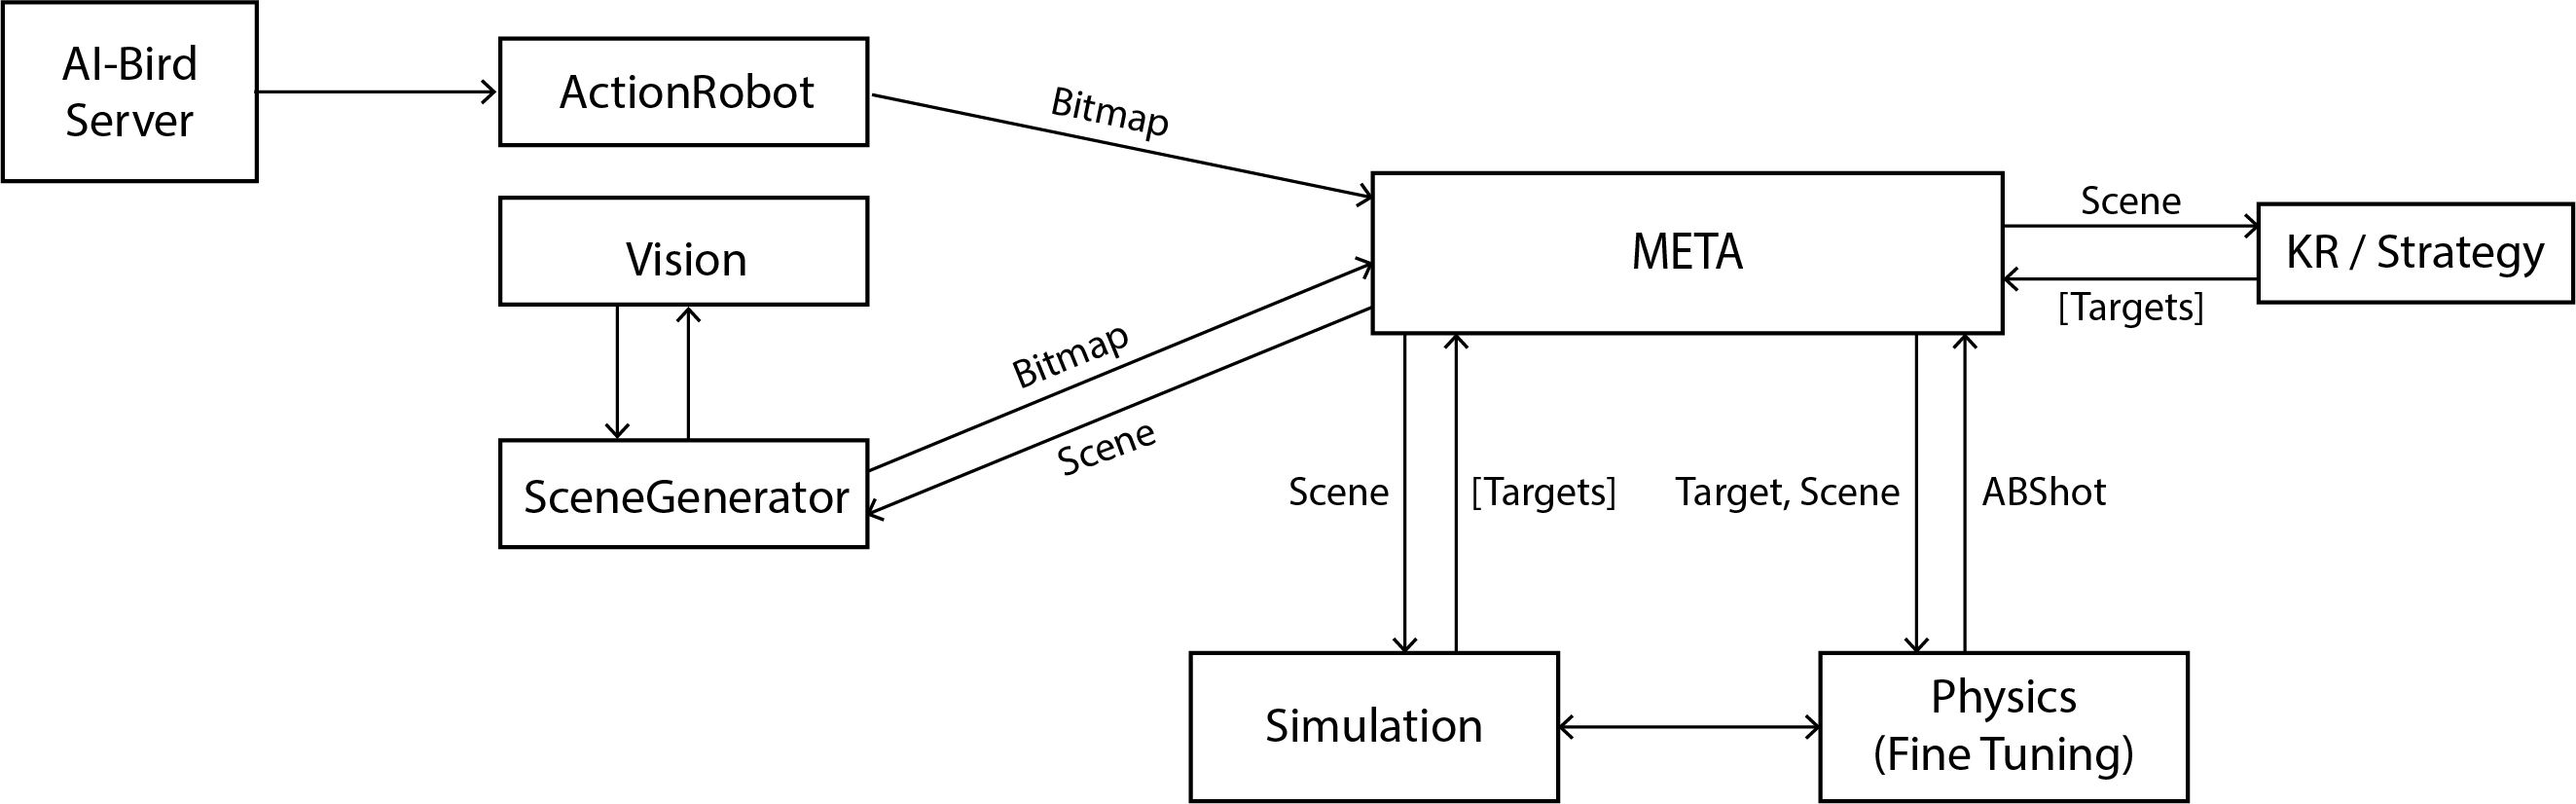
\includegraphics[width=150mm]{ablaufdiagramm.jpg}
		\caption{Wechselspiel der einzelnen Komponenten des Wettbewerbs.}
	\end{center}
\end{figure}

Wir übernahmen die Aufgaben der Meta-Strategie. Diese übergreift alle anderen Komponenten und führt diese Zusammen, ist also eine Art Schnittstelle für die anderen Gruppen.\\
Die Meta-Strategie hat sich insbesondere folgenden Arbeitsfeldern angenommen. Als Erstes haben wir uns mit der Auswahl der verschiedenen Level während des Spiels beschäftigt. So nehmen wir Einfluss auf den Spielfluss und entscheiden in welcher Reihenfolge und wie oft die einzelnen Level gespielt werden sollen.
Eine weitere wichtige Aufgabe ist es, die richtigen Aktionen auszuwählen. Wir haben uns in dieser Hinsicht auf die Auswahl der Schüsse spezialisiert. Aus einer Liste, die wir von der Strategie-Gruppe erhalten, wählen wir, den als besten markierten Schuss aus. Zur Vorhersage einer guten Handlung haben wir uns des weiteren eine Form der Evaluation einzelner Schüsse überlegt, um besonders gute Schüsse zu kennzeichnen und diese in ähnlichen Situationen wieder anzuwenden.
Alle Informationen werden zu jedem einzelnen Schuss in einer Datenbank gespeichert, die wir implementiert haben.\\
Genaue Informationen über den Vorgang unserer Implementierung werden im folgenden Kapitel näher ausgeführt.